% ----------------------------------------------------------
% Introdução
% ----------------------------------------------------------

\chapter{Introdução}

Neste capítulo introdutório será feita uma contextualização sobre a evolução da internet, impactos e crescimento tanto das redes sociais quanto vegetarianismo e veganismo, juntamente com a apresentação das justificativas que levaram ao desenvolvimento do aplicativo para dispositivos móveis proposto neste trabalho.

\section{Contextualização}

A Internet nasceu da soma de pequenas conquistas tecnológicas com o passar dos anos. No inicio da década de 90, desde que foi aberta comercialmente, a internet tem passado por grandes mudanças, evoluindo cada vez mais, criando milhares de recursos e possibilidades de facilitar e organizar conteúdos e informações dos mais diversos tipos. É perceptível as enormes transformações que a internet vem causando nas comunicações, no trabalho, no comércio, no entretenimento.

Inicialmente os \textit{sites} surgiram praticamente para o compartilhamento de informações, de uma forma simples e direta, apenas com textos. Anos depois com mais tecnologias disponíveis, os \textit{sites} ja eram mais trabalhados, com mais detalhes em seu \textit{layout}, tendo imagens e cores. Em constante evolução a internet continuou agregando cada vez mais novas funcionalidades, dando espaço para usar novas tecnologias para deixar os sites com mais conteúdos e mais atraentes.

Com o surgimento da Web 2.0, em meados dos anos 2000, que visava atender às necessidades das novas gerações, tornando a internet mais dinâmica, livre e colaborativa, um outro tipo de serviço de comunicação e entretenimento começou a ganhar força: as redes sociais. Rede social significa interação e troca social, compartilhando interesses e conhecimento. O ser humano por natureza sempre busca se comunicar, segundo \citeauthor{oliveira-marta}, “é a necessidade de comunicação que impulsiona, inicialmente, o desenvolvimento da linguagem”.

As redes sociais mudaram a forma como as pessoas avaliam o que acontece ao seu redor. Segundo \citeauthor{patricio-utilizacao}, as redes sociais são aplicações que suportam um espaço comum de interesses, necessidades e metas comuns para a colaboração, partilha de conhecimento, interação e comunicação. Além disso, são excelentes ferramentas que podem ser usadas para promover o pensamento crítico e fornecer oportunidades de debates.

No entanto, as pessoas tendem a ficar cansadas de utilizar o mesmo serviço todos os dias e iniciam uma busca por algo novo. Com isso, surgem as redes sociais de nicho, que estão tendo um destaque cada vez maior na internet. As pessoas estão interessadas em assuntos comuns, e não pretendem abranger um grande número de usuários. 

A procura se deve porque o usuário quer algo mais específico de acordo com suas preferências e não um ambiente em que se fala de tudo, até do que não o agrada. É o caso das pessoas adeptas ao vegetarianismo. É cada vez mais comum, nos círculos de amigos e/ou familiares e nas redes sociais, encontrar pessoas que optaram pelo estilo de vida natural. A busca pela qualidade de vida, compaixão e respeito pelos animais são alguns dos motivos que têm colaborado com o crescimento do vegetarianismo.

No entanto, mesmo com a crescente adesão ao vegetarianismo, nota-se uma grande dificuldade em encontrar produtos de boa procedência, restaurantes, entre outros estabelecimentos. Até mesmo quando se encontrado locais que os vegeterianos possam vir se alimentar, o cardapio se torna limitado, com poucas opções e nem sempre agradam. Diante desses empecilhos, a melhor solução é sempre fazer sua própria alimentação, buscando os diversos tipos e variados de receita vegetarianas e veganas.

Nesse contexto, aplicativos para o nicho vegetariano foram surgindo. Atualmente,  existem alguns aplicativos de receitas culinárias voltado para o vegetarianismo, mas não possuem um foco social, apenas informações já cadastradas para que os usuários possam usufruir, mas sem ter um vinculo social com outros usuários, o que é importante pela necessidade de colaboração, partilha de conhecimento, interação e comunicação.

Tendo em vista as informações apuradas sobre redes sociais, dispositivos móveis , vegetarianismo e veganismos, consideramos neste trabalho o desenvolvimento de uma aplicativo móvel, que permite os usuários disponibilizarem no ambiente virtual seus interesses pessoais e/ou conhecimentos por receitas culinárias vegetarianas, sendo possível o detalhamento completo de uma receita culinária vegetariana e / ou vegana, contendo a inserção de imagens e outras informações pertinentes, de modo a deixá-la simples e de fácil entendimento. Foi realizada uma pesquisa nas principais lojas virtuais, tais como Google Play e Apple Store , onde foram encontrados algumas aplicações voltadas ao nicho vegetariano, mas nenhuma com o intuito social que o presente trabalho venha a apresentar. Veja na tabela abaixo:

\begin{table}[H]
	\centering
	\caption{Alguns aplicativos nas lojas virtuais voltado para o nicho vegetariano e vegano.}
	\label{tabela-aplicativos-vegetarianos-veganos}
	\begin{tabular}{|l|c|c|l|}
	\hline
	\textbf{} & \textbf{Google Play} & \textbf{Apple Store} & \textbf{Descrição} \\ \hline
	21 – Day Vegan Kickstar & - & x & \begin{tabular}[c]{@{}l@{}}Propõe refeições completas \\ por 21 dias\end{tabular} \\ \hline
	I`m Hungry & x & - & \begin{tabular}[c]{@{}l@{}}Contém diversas receitas \\ pré cadastradas\end{tabular} \\ \hline
	Vgan & x & - & \begin{tabular}[c]{@{}l@{}}Seu foco principal são \\ informações sobre bebidas\end{tabular} \\ \hline
	BeVeg & x & x & \begin{tabular}[c]{@{}l@{}}Delivery de restaurante\end{tabular} \\ \hline
	HappyCow & x & x & \begin{tabular}[c]{@{}l@{}}Um guia onde indica \\ restaurantes, bares e lojas\end{tabular} \\ \hline
	\end{tabular}
\end{table}

É importante ressaltar que, como o ambiente da aplicação é uma rede social , essas informações serão compartilhadas por todos os usuários da rede, por meio de uma timeline ou linha do tempo, na qual poderão ver todas as publicações de todos os demais usuários adicionados na sua rede. 

\section{Justificativa}

De acordo com um relatório realizado pelo \citeauthor{eMarketer}, em 2017 pelo menos 71\% dos internautas em todo o mundo terão acesso a redes sociais, como pode ser visto por meio da  Figura \ref{fig:figura1}.

\begin{figure}[H]
	\caption{\label{fig:figura1}Usuários de rede social e penetração em todo o mundo.}
	\centering
	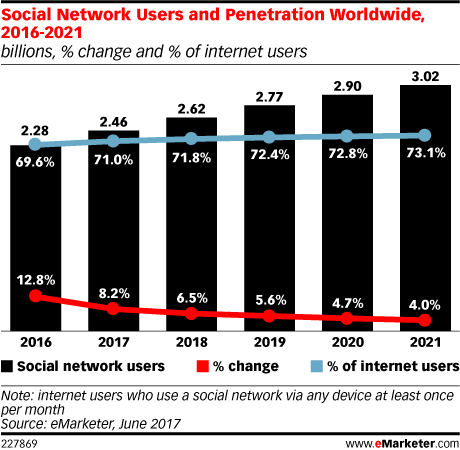
\includegraphics[scale=0.5]{imagens/figura1.png}
	\legend{Fonte: \citeauthor{eMarketer}}
\end{figure}

Com a expansão das redes sociais, o uso de dispositivos móveis vem crescendo consideravelmente no mundo. Em 2014 o acesso à internet por meio de dispositivos móveis superou o acesso por meio de desktops, como pode ser visto na Figura \ref{fig:figura2}.

\begin{figure}[H]
	\caption{\label{fig:figura2}Projeção Global de usuários de desktop vs. usuários de internet móvel.}
	\centering
	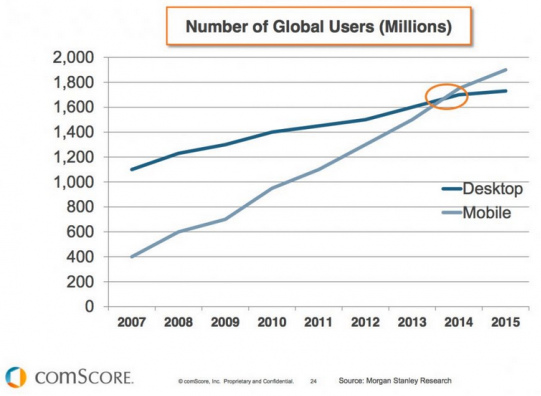
\includegraphics[scale=0.5]{imagens/figura2.png}
	\legend{Fonte: \citeauthor{smartinsights}}
\end{figure}

A \citeauthor{svb} - Sociedade Vegetariana Brasileira, divulgou uma pesquisa realizada pelo Instituto Brasileiro de Opinião Pública e Estatística, IBOPE, que 15,2 milhões de brasileiros se declaram vegetarianos, isso corresponde a 8\% da população do país. De acordo com o Google Trends, de Janeiro de 2012 a Julho de 2016 o volume de buscas pelo termo ‘vegano’ cresceu 1000\% (mil por cento) no Brasil.

Assim, existe uma necessidade preemente de mobile + redes sociais + veganismo/vegetarianismo, surgindo a ideia da criação de um aplicativo envolvendo essas três conceitos.
 
\section{Objetivos}

Nesta seção serão apresentados o objetivo geral e os específicos do presente trabalho.

\subsection{Objetivo Geral}

Desenvolver uma rede social de receitas culinárias vegetarianas e veganas, implementada em uma ferramenta tecnológica híbrida , que poderá funcionar nos sistemas operacionais mais utilizados atualmente: Android e IOS.

\subsection{Objetivos Específicos}
\begin{lista}
  \item Apresentar o referencial teórico sobre as tecnologias a serem utilizadas;
  \item Desenvolver análise e projeto do sistema proposto como estudo de caso;
  \item Codificar o aplicativo utilizando técnicas apropriadas através o framework Ionic;
  \item Realizar teste de usabilidade da interface criada, para que possa ter um resultado satisfatório e eficaz;
  \item Disponibilizar para o usuário uma versão do aplicativo para download (Google Play).
\end{lista}